\documentclass[notoc,justified,openany]{tufte-book}    % `notoc` suppresses TL custom TOC, reverts to standard LaTeX
\usepackage{graphicx}
\usepackage{xspace}
\hyphenation{HMMER}
\newcommand{\hmmer}{{HMMER}\xspace}  % \hmmer is a command that expands to "HMMER" with a trailing space
\newcommand{\hmmot}{{HMMot}\xspace}  % \HMMot is a command that expands to "HMMot" with a trailing space
\newcommand{\userguide}{HMMER User's Guide}
\title{User's Guide for the HMMot viewer for HMMER results}

\subtitle{High-performance biological sequence analysis using profile hidden Markov models}

\author{Nicholas P. Carter, Sean R. Eddy}
\subauthor{and the HMMER development team}

\pkgurl{http://hmmer.org}
\pkgversion{3.4}   % ./configure replaces HMMER_VERSION
\pkgdate{June, 2025}         %    ... and HMMER_DATE

                    % definitions for \maketitle 
\bibliographystyle{unsrtnat-brief}   % customized natbib unsrtnat. Abbrev 3+ authors to ``et al.'' 

\begin{document}
\setcounter{tocdepth}{2}             % 0=chapters 1=sections 2=subsections 3=subsubsections? 4=paragraphs

\maketitle

\newpage
\begin{fullwidth}
  ~\vfill
  \thispagestyle{empty}
  \setlength{\parindent}{0pt}
  \setlength{\parskip}{\baselineskip}

\par
Copyright (C) 2026 Howard Hughes Medical Institute.

\par
HMMER and its documentation are freely distributed
under the 3-Clause BSD open source license. For a copy of the license,
see \href{https://opensource.org/licenses/BSD-3-Clause}{opensource.org/licenses/BSD-3-Clause}.

\par
HMMER development is supported in part by the National Human
Genome Research Institute of the US National Institutes of Health under
grant R01HG009116. The content is solely the responsibility
of the authors and does not necessarily represent the official views of
the National Institutes of Health.

\end{fullwidth}







\pagebreak
\hspace{0pt}
\vfill
\emph{\hmmot is dedicated to the memory of Tom Jones: biologist, friend, and Player of Games. Tom was one of the inspirations for the development of \hmmot, but passed away before it was completed.  We hope that \hmmot will help others bring the curiosity, thoughtfulness, and joy to biology that Tom showed every day.}
\vfill
\hspace{0pt}

\chapter{Introduction}
The size of modern genomic datasets makes parsing the results of \hmmer and other homology search tools challenging.  \hmmer searches often locate thousands of homologs to a query sequence or HMM, with a few outliers locating millions of related sequences.  As examining each of these results by hand would take an impractical amount of time, there is a need for a tool that displays the results of a \hmmer search in a way that allows the user to quickly understand the distribution of the homologs to a query sequence or HMM and then focus on the homologs that are of greatest interest.  \hmmot\sidenote{HMMER Observation Tool, also a thinly-disguised reference to Tom Jones} is intended to meet this need by categorizing homologs according to their \emph{domain structure}, a canonicalized representation of the domains found in a sequence.  Sorting search results this way provides users with an easy-to-parse overview of the different types of homologs a search has found that they can then investigate to better understand the categories that most interest them.

\hmmot was heavily inspired by the work done by our collaborators at the European Bioinformatics Institute (EBI) on their web-accessible HMMER server which can be found at \url{https://www.ebi.ac.uk/tools/hmmer/}.  Many of our users found the results display on the web server useful enough that they would run searches there instead of on our local machines, motivating us to develop \hmmot to bring this capability to anyone with access to \hmmer.

\section{Domain Structures}
A sequence's \emph{domain structure} is an ordered list of the domains that the sequence contains, modified as necessary to remove overlapping domains so that the domain structure can be displayed on a single line.  The algorithm we use to remove overlaps is:
\begin{enumerate}
  \item{Sort the domains in a sequence in ascending order of start position.}
  \item{Proceed through the list of domains, checking to see if any pair overlaps.}
  \item{If two sequences are found to overlap by a small number of positions (5 or fewer residues), shrink the sequence with the higher (worse) e-value to eliminate the overlap, which may eliminate it completely.}
  \item{If two domains overlap by more than five residues and the domains are members of the same clan, delete the domain with the higher e-value.  If they are not members of the same clan, shrink the sequence with the higher e-value to eliminate the overlap. }
\end{enumerate}

\chapter{Installation}
Unlike the main {HMMER} package, \hmmot is primarially distributed in binary (executable) form.  This is because \hmmot makes use of a number of open-source libraries to reduce development effort, making building it from source more complex than the rest of {HMMER}, which goes to great lengths to avoid depending on any other software.  \hmmot remains an open-source tool, and source code can be found at (location TBD).  

To install \hmmot, download the appropriate package for your operating system from (place), unzip/untar the file, and place the \hmmot executable either somewhere in your {PATH}, if on a {UNIX} system, or in the Applications directory, if on a Mac\sidenote{This is not strictly necessary, as \hmmot can be run from anywhere, but will make it easier to locate and run the application.}.  You will also need one or more annotated sequence databases that provide the domain information that \hmmot uses.  We provide a number of such databases at (location), and this manual contains instructions for annotating your own databases.


\chapter{Usage}
\hmmot requires two inputs: the output of one or more \texttt{hmmsearch} or \texttt{phmmer} searches, and an annotated version of the sequence database the search(es) were run against.  The search outputs must be in the format generated by the \texttt{-{}-domtblout} option of \texttt{hmmsearch} or \texttt{phmmer}, and will be referred to as "domtblout files".  The annotated database contains information about the domains contained in each sequence as well as the orginization of domains into clans\sidenote{While this document assumes the common case where a sequence database is annotated with the set of Pfam domains that hit each of its sequences, our tools allow annotating a sequence database based on matches to any set of {HMMs} the user provides.}

When first started, \hmmot begins at the "load data" screen, as shown in Figure \ref{fig:load-data}. The top and bottom of the screen contain several elements that appear on all of {HMMot's} screens.  At the top left, the "hamburger" icon consisting of three horizontal lines allows one to bring up {HMMot's} menu, from which one can view information about \hmmot or quit the application.  At the top right, clicking the gear icon will bring up the settings screen, where one can choose the font that \hmmot uses, select a light or dark theme, choose a scaling factor for text, and select the maximum e-value and domain e-value of hits that \hmmot should display.  All settings are saved out to a configuration file so that \hmmot retains its appearance on subsequent runs.

\begin{figure*}
\centering
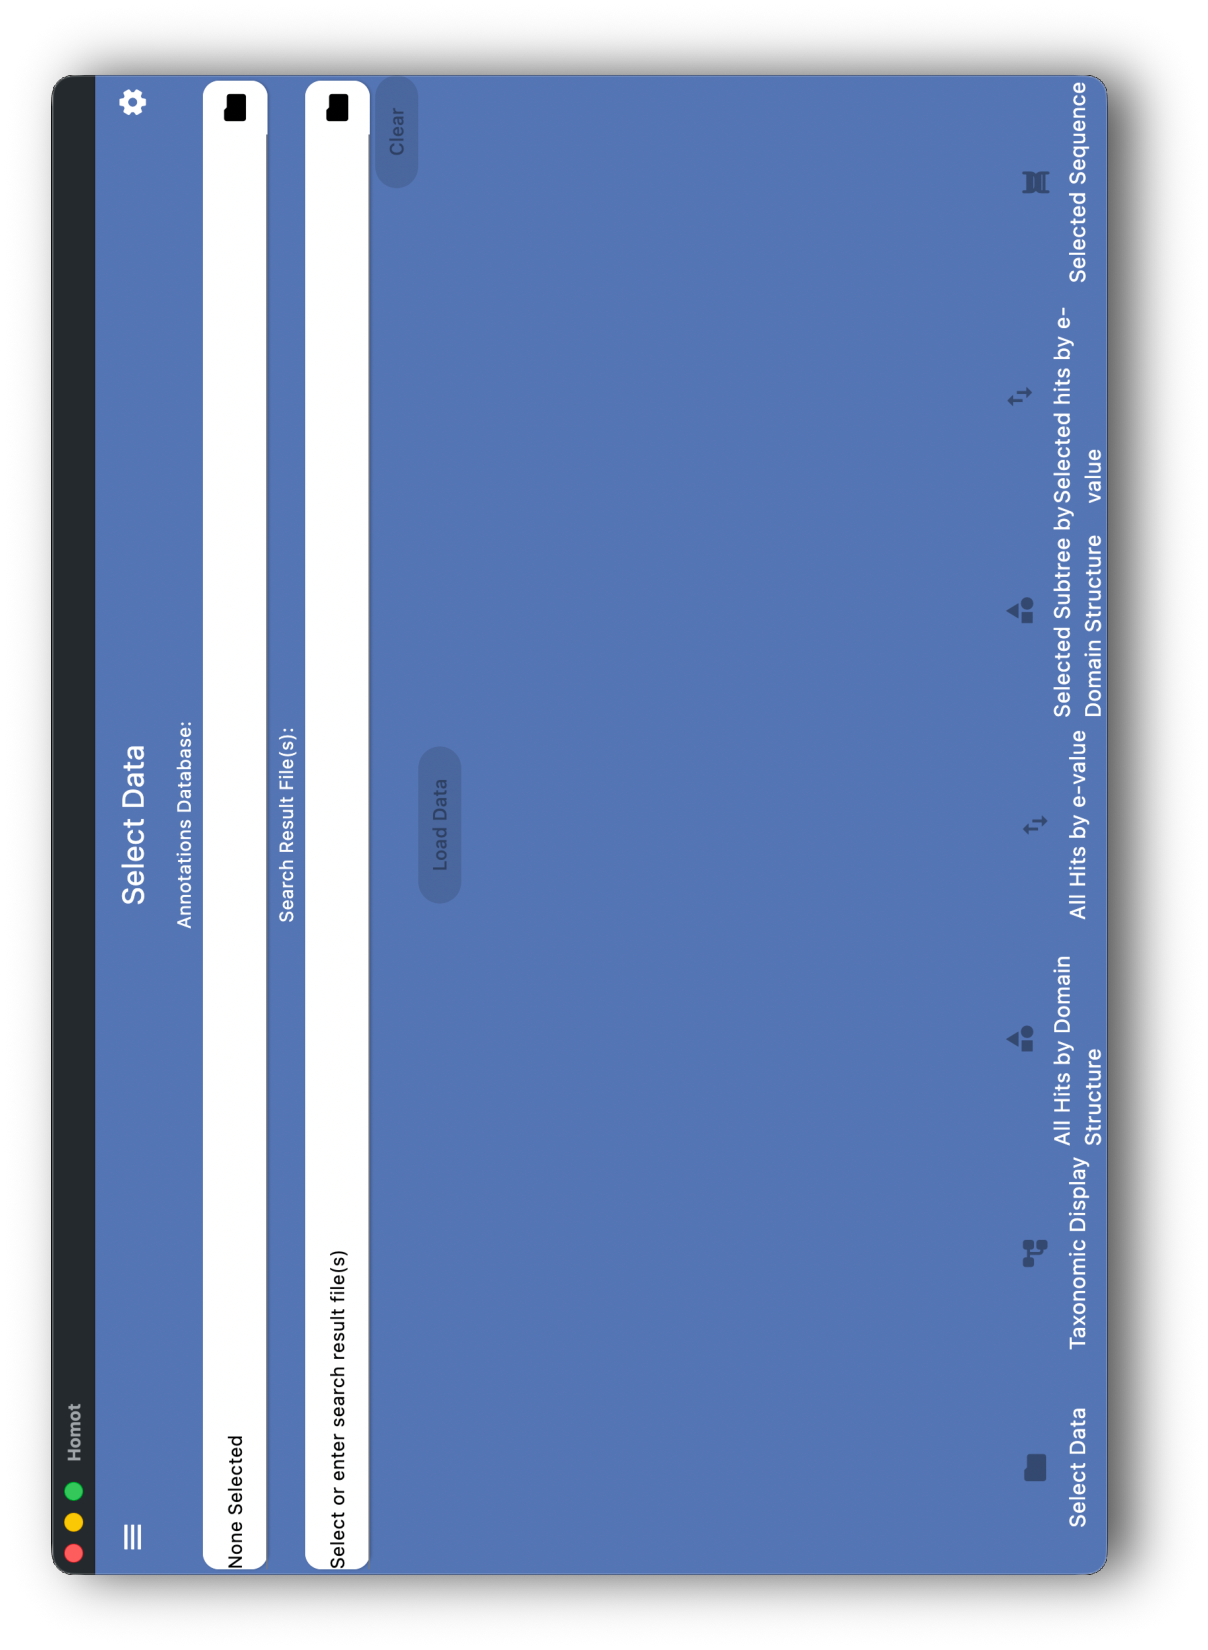
\includegraphics[width=\textwidth]{inclusions/load_data.pdf}
\caption{Load Data Screen}
\label{fig:load-data}
\end{figure*}

At the bottom of the screen, the navigation bar allows the user to switch between {HMMot's} four main screens: the "load data" screen, a screen that displays a summary of all selected search results, a screen that displays all hits with a selected domain structure, and a screen that shows the details of a particular sequence.  Initially, all of these options are greyed out and unavailable because \hmmot is on the "load data" screen and it is not possible to switch to any of the data display screens until data has been loaded.  As data is loaded, a domain architecture selected to view, and/or a sequence selected to focus on, the navigation buttons will become active, allowing switching between screens.

In the center of the screen, fields allow the user to select the annotated database that \hmmot will use and one or more domtblout files of search results to display.  This can be done either by entering the path to the data in the fields, or by clicking the file icon at the right to bring up a file picker.  Note that the annotated databases \hmmot uses are a directory containing multiple files, and \hmmot should be given the location of that directory, not any of the files it countains.  Once both an annotated database and one or more domtblout files have been selected, the "Load Data" button will become active and can be clicked to load search results into \hmmot.

Once loading completes, \hmmot will switch to the "All Results" screen, shown in Figure \ref{fig:overview} which shows a summary of all of the hits in the selected domtblout file(s).  Hits are grouped by domain structure, and the domain structures are sorted from the one with the most hits to the one with the fewest.  If there are more different domain structures than can be displayed simultaneously, a scrollbar on the right side of the window can be used to browse the full list.  

\begin{figure*}
\centering
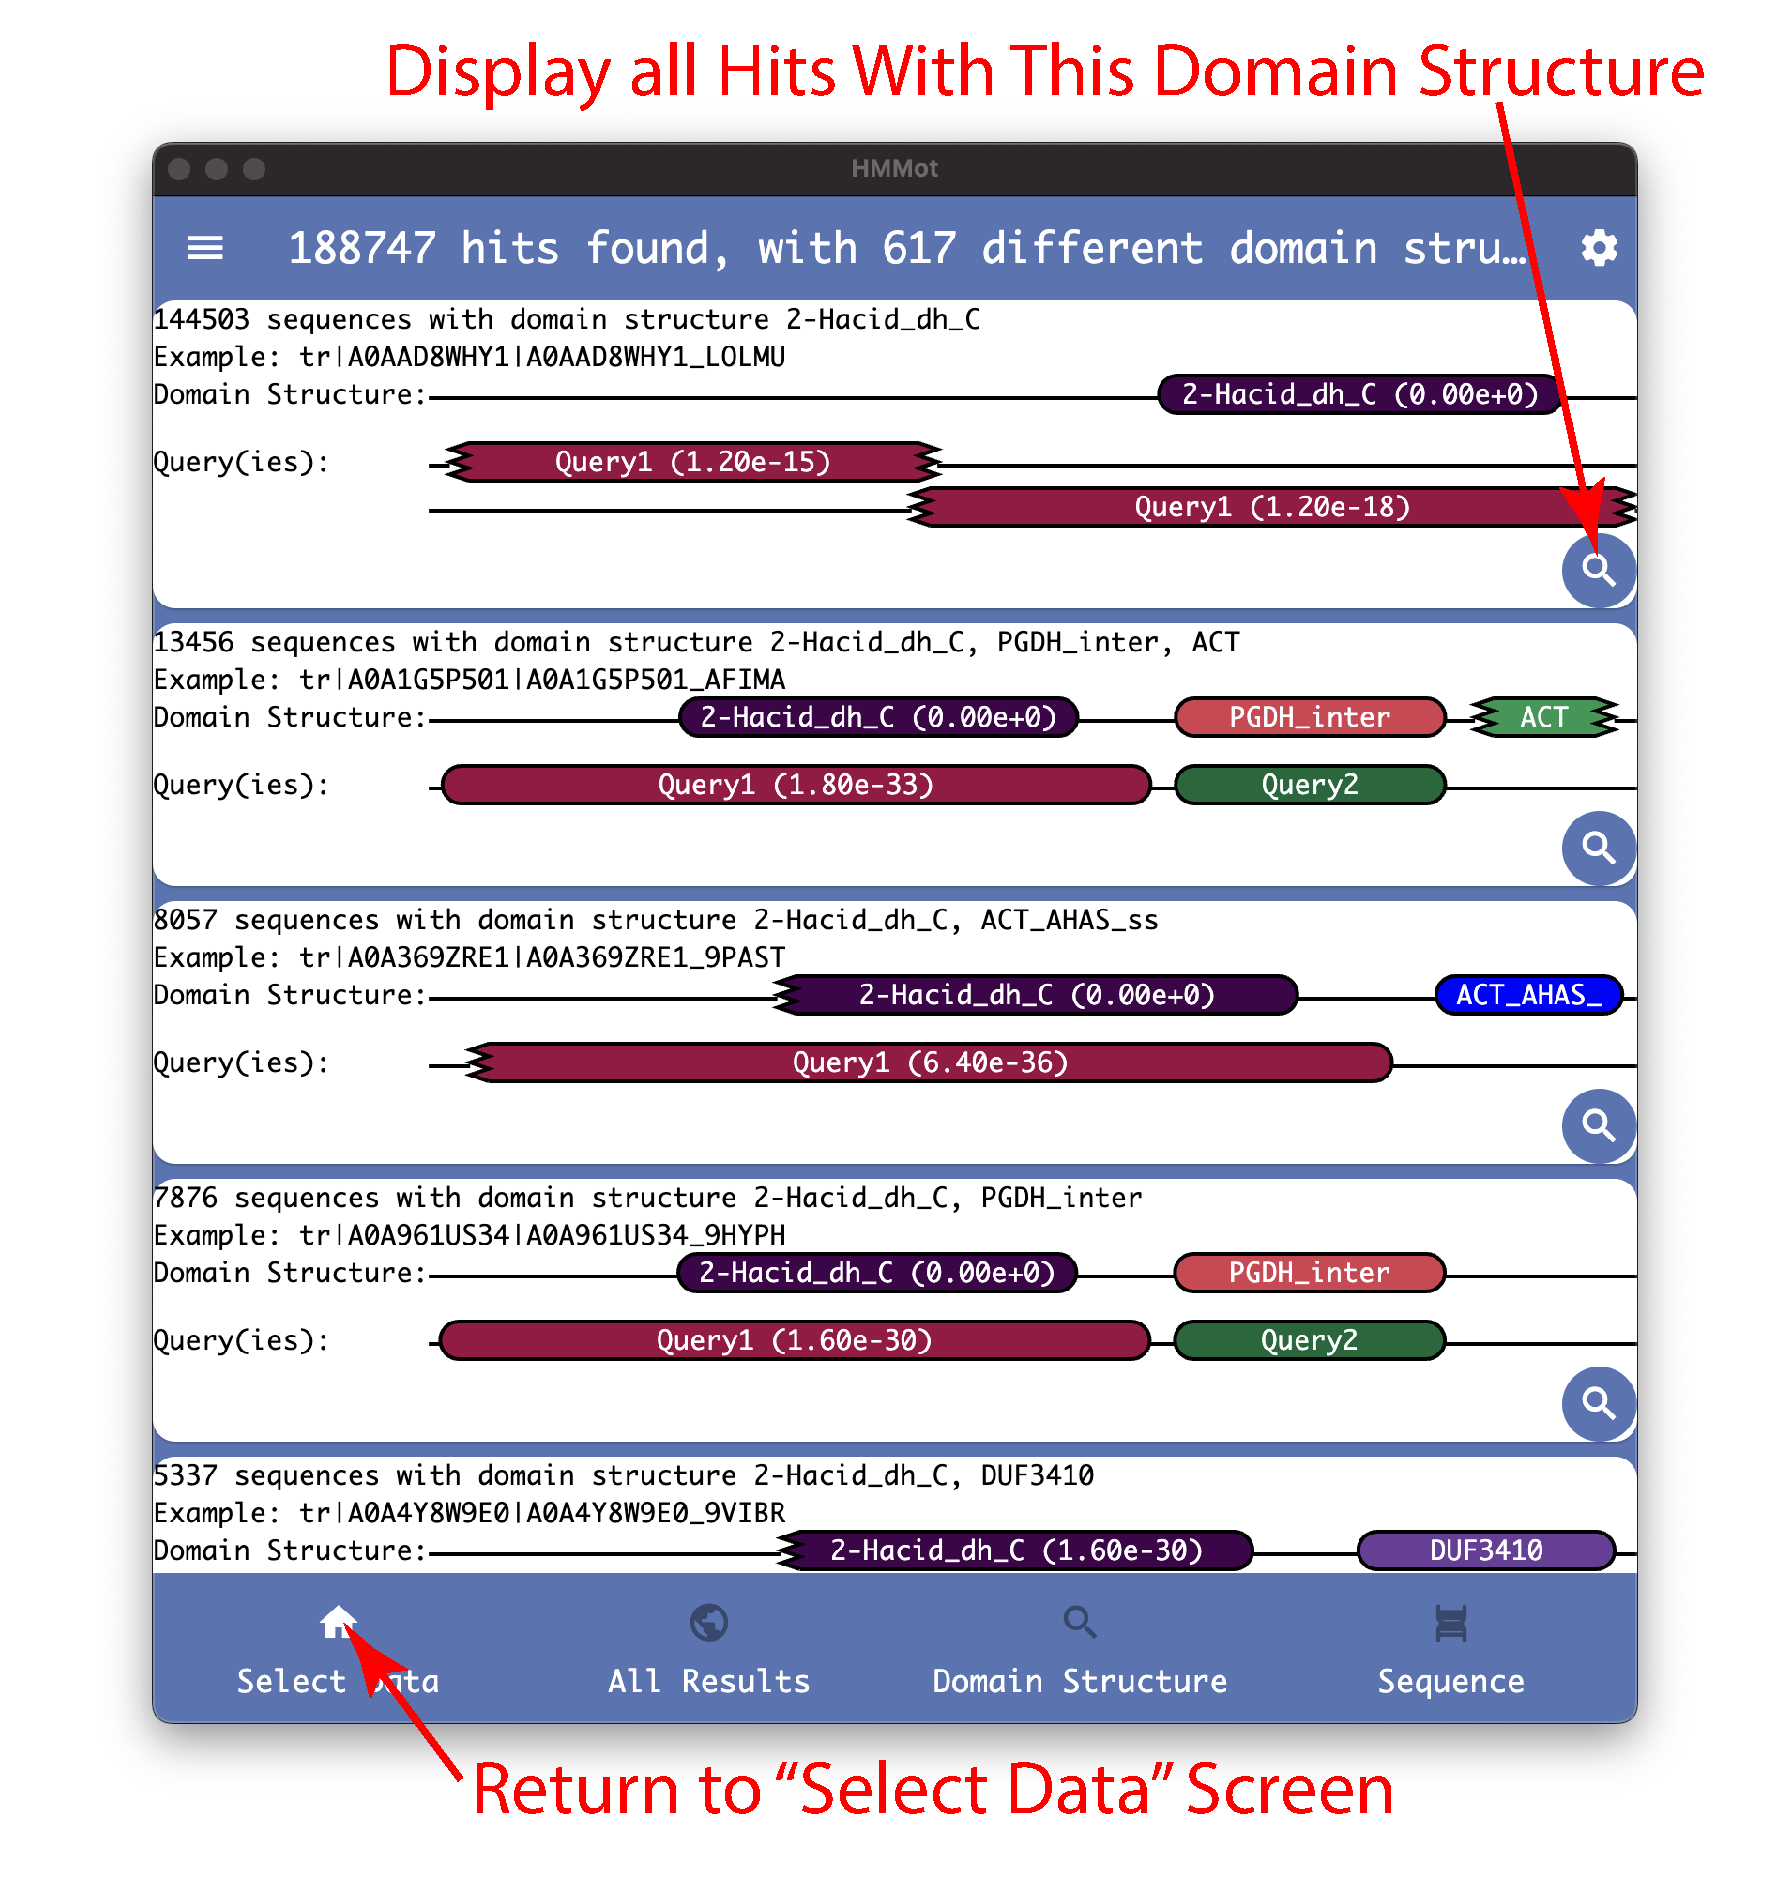
\includegraphics[width=\textwidth]{inclusions/overview.pdf}
\caption{Results Overview Screen}
\label{fig:overview}
\end{figure*}

For each different domain structure, \hmmot shows the number of hits with that domain structure and displays the details of an example hit (the one with the best e-value) that has that structure.  The domain structure of the example hit is illustrated, along with the locations of the hit(s) that the query or queries being shown had to the example sequence.  Hits and domains are colored using a rotating palette of 20 foreground/background color combinations to help distinguish them.  If there is enough space, each hit or domain shows the full name of the query or domain, along with the e-value of that hit or domain.  If not, the information is truncated to fit the available space.  

Rounded edges at the beginning or end of a hit/domain indicate that the match of the hit/domain extended to the beginning or end of the HMM, while jagged edges indicate that the match started or ended in the middle of the HMM.  A hit or domain with square edges indicates that there was not room to show any text describing the hit or domain.  In all cases, mousing over a hit or domain will display more detailled information about it. 
\begin{figure*}
\centering
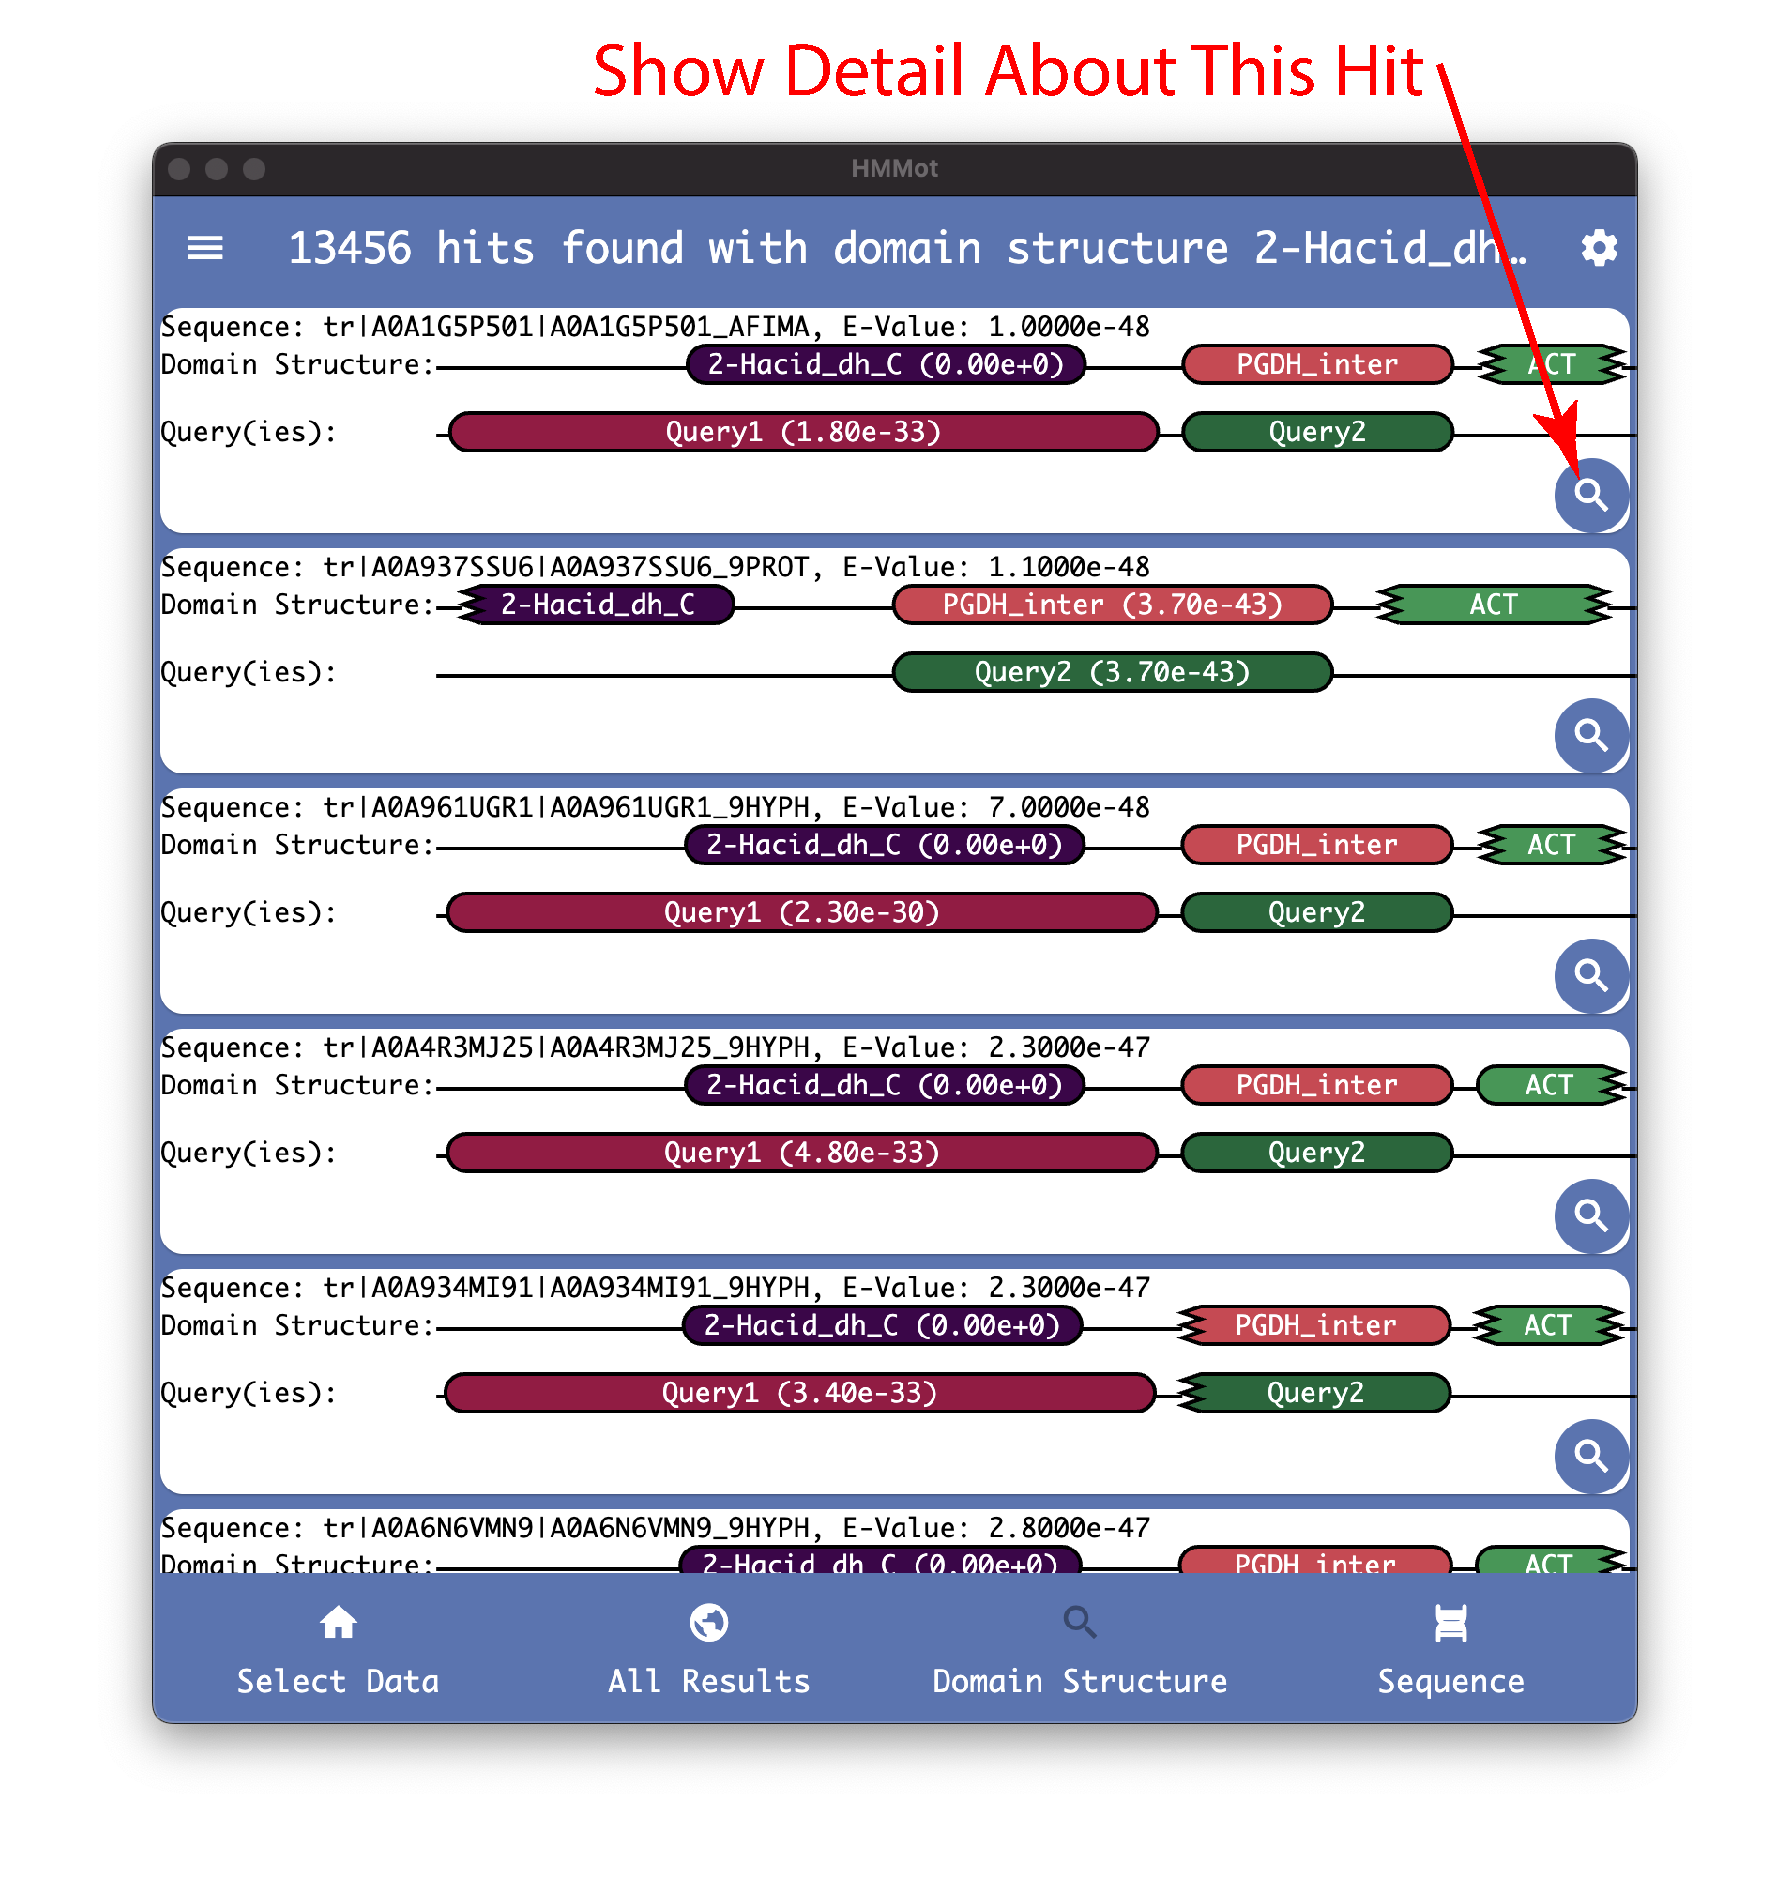
\includegraphics[width=\textwidth]{inclusions/domain_structure.pdf}
\caption{Domain Structure Screen}
\label{fig:domain_structure}
\end{figure*}

Clicking on the magnifying glass icon at the bottom right of the information about the hits with a given domain architecture will bring up the "Domain Structure" screen, as shown in \ref{fig:domain_structure}, which shows all of the hits with the specified domain architecture, sorted in ascending order by e-value.  Each sequence shows the domain structure of the sequence, along with the position of the hit or hits. 

Finally, clicking the magnifying glass in the lower right of a given sequence's information will bring up a screen with detailled information about the sequence, as shown in \ref{fig:sequence}. This screen shows all of the domains that the sequence was annotated with, not just the domain structure, as well as showing the sequence itself.

\begin{figure*}
\centering
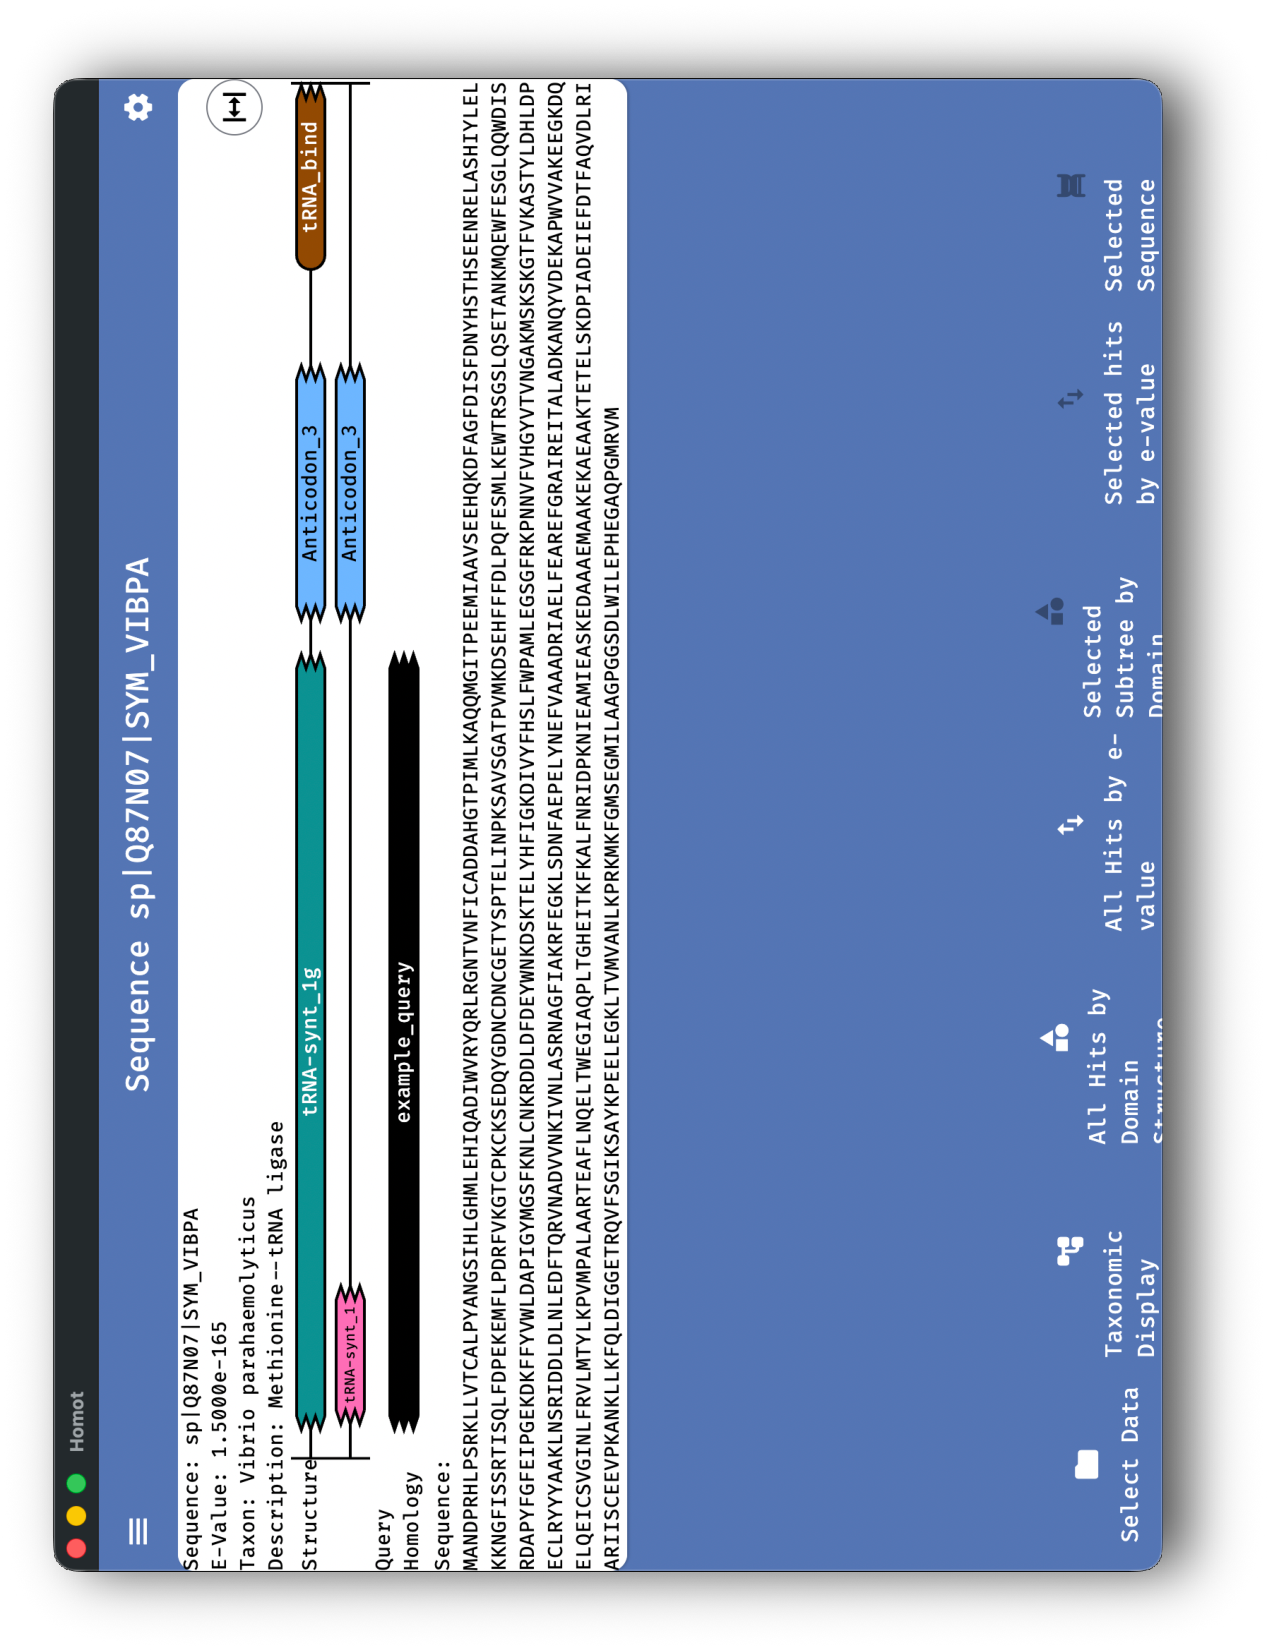
\includegraphics[width=\textwidth]{inclusions/sequence.pdf}
\caption{Sequence Screen}
\label{fig:sequence}
\end{figure*}

\section{Annotating a Sequence Database}
While we provide annotated versions of some sequence databases at (location), users may wish to annotate their own databases, and we provide the tools to do this.  While our methodology is mainly intended to annotate databases with the set of domains defined by Pfam~\url{http://pfam.xfam.org/}, it can be adapted to annotate databases with the results of any set of searches you desire.

Annotating a database requires four inputs:
\begin{enumerate}
  \item{The sequence database you wish to annotate, }
  \item{A directory containing domtblout files generated by running \mono{hmmsearch} on one or more HMMs that characterize the domains you wish to annotate.  Each domtblout file should contain the results of searching one HMM against the database.}
  \item{A single hmmfile containing all of the HMMs used in generating the domtblout files.}
  \item{A file that defines the relationships between domains and clans.  This can be the "Pfam-A.clans.tsv" file that Pfam provides if you are annotating a database with the Pfam domains.  Otherwise, it should be a tab-separated value (tsv) file, containing four fields for each domain: A numeric ID in the form "PFXXXXX", a numeric ID for the clan the domain belongs to, in the form "CLXXXXX", the name of the clan, and the name of the domain.  If the domain does not belong to a clan, the second and third fields can be blank, but the file must still have four columns per line (i.e., there must be three tab characters to separate the fields, even if some of the fields are empty.). Note that \hmmot uses 16-bit integers to hold domain and clan identifiers, so is only able to support 65,536 domains or clans.}
\end{enumerate}

Once these inputs are available, run the \texttt{create-annotations} program that we provide to create an annotated version of the database.  Because \texttt{create-annotations} keeps its intermediate state in memory until it has fully-annotated the database, it can use significant amounts of RAM.  Annotating a large database also takes a non-trivial amount of time, approximately 24 hours for a database with 200M sequences.



\chapter{Acknowledgements}

We are deeply indebted to the HMMER server team at the European Bioinformatics Institute, whose work on web tools to display HMMER search results was the inspiration for \hmmot.  We would also like to thank all those who provided feedback and comments on early versions of \hmmot. This work was supported by the Howard Hughes Medical Institute and the National Institutes of Health, under grant R01HG009116.

\hmmot is based on a number of freely-licensed and/or open-source software packages. Chief among these are Flutter~\url{https://flutter.dev} and Dart~\url{https://dart.dev}, the GUI toolkit and language used to implement most of \hmmot. Portions of \hmmot were written in Rust~\url{https://www.rust-lang.org/}, with the help of the Flutter-Rust Bridge ~\url{https://github.com/fzyzcjy/flutter_rust_bridge} package.

\hmmot incorporates a number of Flutter and Dart packages, including File Picker~\url{https://pub.dev/packages/file_picker}, Go Router~\url{https://pub.dev/packages/go_router}, Hive~\url{https://pub.dev/documentation/hive/latest/}, Input Quantity~\url{https://pub.dev/packages/input_quantity}, Osler Icons~\url{https://pub.dev/packages/osler_icons}, Provider~\url{https://pub.dev/packages/provider}, Shared Preferences~\url{https://pub.dev/packages/shared_preferences}, System Fonts~\url{https://pub.dev/documentation/system_fonts/latest/}, and Touchable~\url{https://pub.dev/packages/touchable/versions}.  Licenses for these and other packages that Dart and Flutter incorporate can be found by selecting "About" from {HMMot's} menu and clicking the "View Licenses" button on the dialog that appears.

Our Rust code depends on the Bio~\url{https://docs.rs/bio/latest/bio/}, Dashmap~\url{https://docs.rs/dashmap/latest/dashmap/}, Fjall~\url{https://docs.rs/fjall/latest/fjall/}, Glob~\url{https://docs.rs/glob/latest/glob/}, Rayon~\url{https://docs.rs/rayon/latest/rayon/}, Rmp-serde~\url{https://docs.rs/rmp-serde/latest/rmp_serde/}, and Serde~\url{https://docs.rs/serde/latest/serde/} crates, all of which are released under the MIT license. 


\end{document}